
\documentclass[
% -- opções da classe memoir --
12pt,				% tamanho da fonte
openright,			% capítulos começam em pág ímpar (insere página vazia caso preciso)
oneside,			% para impressão em recto e verso. Oposto a oneside
a4paper,			% tamanho do papel. 
% -- opções da classe abntex2 --
chapter=TITLE,		% títulos de capítulos convertidos em letras maiúsculas
section=TITLE,		% títulos de seções convertidos em letras maiúsculas
%subsection=TITLE,	% títulos de subseções convertidos em letras maiúsculas
%subsubsection=TITLE,% títulos de subsubseções convertidos em letras maiúsculas
% -- opções do pacote babel --
english,			% idioma adicional para hifenização
french,				% idioma adicional para hifenização
spanish,			% idioma adicional para hifenização
brazil				% o último idioma é o principal do documento
]{abntex2-uepg}

% ---
% Pacotes básicos 
% ---
\usepackage{lmodern}			% Usa a fonte Latin Modern			
\usepackage[T1]{fontenc}		% Selecao de codigos de fonte.
\usepackage[utf8]{inputenc}		% Codificacao do documento (conversão automática dos acentos)
\usepackage{indentfirst}		% Indenta o primeiro parágrafo de cada seção.
\usepackage{color}				% Controle das cores
\usepackage{graphicx}			% Inclusão de gráficos
			% para melhorias de justificação]
\usepackage{uepg}
\usepackage{lipsum}		
\usepackage{amssymb}
\usepackage{amsmath}
%\usepackage{paralist}
\usepackage{setspace}
\usepackage{lscape}
\usepackage{longtable}	
\usepackage{listings}
\usepackage{gantt}
\usepackage{inconsolata}
\usepackage{xcolor}
\usepackage[bottom=2cm,top=3cm,left=3cm,right=2cm]{geometry}
\usepackage{titlesec}
\usepackage{caption}
\captionsetup[table]{
	singlelinecheck=false, % Alinha o caption à esquerda
}
\captionsetup[figure]{
	singlelinecheck=false, % Alinha o caption à esquerda
}
\titlespacing*{\subsection}{0pt}{2.5ex plus 1ex minus .2ex}{2.5ex plus .2ex} 

\setlength\afterchapskip{\lineskip}

\definecolor{codegreen}{rgb}{0,0.6,0}
\definecolor{codegray}{rgb}{0.5,0.5,0.5}
\definecolor{codepurple}{rgb}{0.58,0,0.82}
\definecolor{backcolour}{rgb}{0.95,0.95,0.92}

\lstdefinestyle{mystyle}{
	backgroundcolor=\color{backcolour},   
	commentstyle=\color{codegreen},
	keywordstyle=\color{magenta},
	numberstyle=\tiny\color{codegray},
	stringstyle=\color{codepurple},
	basicstyle=\ttfamily\footnotesize,
	breakatwhitespace=false,         
	breaklines=true,                 
%	captionpos=b,                    
	keepspaces=true,                 
	numbers=left,                    
	numbersep=5pt,                  
	showspaces=false,                
	showstringspaces=false,
	showtabs=false,                  
	tabsize=2,
	frame=single
}

\lstset{style=mystyle}

\usepackage[brazilian,hyperpageref]{backref}	 % Paginas com as citações na bibl
\usepackage[alf,
abnt-emphasize = bf, % destaca o titulo da revista ou livro em negrito;
abnt-etal-list = 3, % trabalhos com mais de 3 autores recebem et al.,;
abnt-etal-text = it, % escreve o et al., em italico;
abnt-and-type = &, % usa o carater '&' no lugar de 'e' para mais de um autor;
abnt-last-names = abnt, % trata sobrenomes 'estritamente' conforme a ABNT; e
abnt-repeated-author-omit = no] {abntex2cite}

% ---
% Configurações do pacote backref
% Usado sem a opção hyperpageref de backref
\renewcommand{\backrefpagesname}{Citado na(s) página(s):~}
% Texto padrão antes do número das páginas
\renewcommand{\backref}{}
% Define os textos da citação
\renewcommand*{\backrefalt}[4]{
	\ifcase #1 %
	Nenhuma citação no texto.%
	\or
	Citado na página #2.%
	\else
	Citado #1 vezes nas páginas #2.%
	\fi}%
% ---
% -- ljsenger
\renewcommand{\rmdefault}{phv} % Arial
\renewcommand{\sfdefault}{phv} % Arial

% formatacao de codigo fonte
\renewcommand{\lstlistingname}{Código}
\renewcommand{\lstlistlistingname}{Lista de códigos}

% ---
% Informações de dados para CAPA e FOLHA DE ROSTO
% ---

\titulo{TITULO DO TRABALHO}
\autor{NOME DO MESTRANDO(A)}
\orientador{Prof. Dr. Orientador}
% \orientador [Orientadora: ]{Prof. Dr. Orientador} caso a orientação seja feminina.
\coorientador{Prof. Dr. Coorientador}
\data{2026}
\local{Ponta Grossa}
\preambulo{Projeto de Dissertação apresentado ao Programa de Pós-Graduação em Computação Aplicada, curso de Mestrado em Computação Aplicada da Universidade Estadual de Ponta Grossa, como requisito parcial para obtenção do título de Mestre.}
\area{Area do projeto}
\linha{Linha de pesquisa}
\ingresso{XX/2025}
\bolsista{Não}

	
\tipotrabalho{Trabalho de Conclusão de Curso}

\definecolor{blue}{RGB}{41,5,195}

\makeatletter
\hypersetup{
	%pagebackref=true,
	pdftitle={\@title}, 
	pdfauthor={\@author},
	pdfsubject={\imprimirpreambulo},
	pdfcreator={LaTeX with abnTeX2},
	pdfkeywords={abnt}{latex}{abntex}{abntex2}{trabalho acadêmico}, 
	colorlinks=true,       		% false: boxed links; true: colored links
	linkcolor=black,          	% color of internal links
	citecolor=black,        		% color of links to bibliography
	filecolor=magenta,      		% color of file links
	urlcolor=black,
	bookmarksdepth=4
}
\makeatother
% --- 

% ---
% Posiciona figuras e tabelas no topo da página quando adicionadas sozinhas
% em um página em branco. Ver https://github.com/abntex/abntex2/issues/170
\makeatletter
\setlength{\@fptop}{5pt} % Set distance from top of page to first float
\makeatother
% ---

% ---
% Possibilita criação de Quadros e Lista de quadros.
% Ver https://github.com/abntex/abntex2/issues/176
%
\newcommand{\quadroname}{Quadro}
\newcommand{\listofquadrosname}{Lista de quadros}

\newfloat[chapter]{quadro}{loq}{\quadroname}
\newlistof{listofquadros}{loq}{\listofquadrosname}
\newlistentry{quadro}{loq}{0}


% configurações para atender às regras da ABNT
\setfloatadjustment{quadro}{\centering}
\counterwithout{quadro}{chapter}
\renewcommand{\cftquadroname}{\quadroname\space} 
\renewcommand*{\cftquadroaftersnum}{\hfill--\hfill}

\setfloatlocations{quadro}{hbtp} % Ver https://github.com/abntex/abntex2/issues/176
% ---

% --- 
% Espaçamentos entre linhas e parágrafos 
% --- 

% O tamanho do parágrafo é dado por:
\setlength{\parindent}{1.3cm}

% Controle do espaçamento entre um parágrafo e outro:
\setlength{\parskip}{0.2cm}  % tente também \onelineskip

%ljsenger - espaçamento simples (e feio) entre parágrafos
\setlength{\parskip}{0cm}
%ljsenger - espaçamento entre o título e o primeiro parágrafo do texto
\setlength\afterchapskip{18pt}

% compila o indice
\makeindex
% ---
% padrão UEPG - fonte ARIAL (ou times)
\renewcommand{\rmdefault}{phv} % Arial
\renewcommand{\sfdefault}{phv} % Arial

\newlistof{lstlistoflistings}{lol}{\lstlistlistingname}
\begin{document}
	
	\selectlanguage{brazil}
	\frenchspacing 
	
	\imprimirfolhaderosto
	
		% ---
	% LISTA DE FIGURAS 
  %%%% Não é necessário alterar essa área, pois os dados são coletados automaticamente na adição de figuras 
  %%%% há um exemplo em 104.revisaoliteratura.tex
	% ---
	\renewcommand{\listfigurename}{Lista de figuras}
	\pdfbookmark[0]{\listfigurename}{lof}
	\listoffigures*
	\cleardoublepage
  % ---  
  
	% ---
	% LISTA DE QUADROS
	% ---
	\pdfbookmark[0]{\listofquadrosname}{loq}
	\listofquadros*
	\cleardoublepage
	% ---
  
	% ---
	% LISTA DE TABELAS
  %%%% Não é necessário alterar essa área, pois os dados são coletados automaticamente na adição de tabelas.
  %%%% há um exemplo em 105.materialemetodos.tex
	% ---
	\pdfbookmark[0]{\listtablename}{lot}
	\listoftables*
	\cleardoublepage
  % ---


  % ---
	% LISTA DE CÓDIGOS FONTE
  %%%% Não é necessário alterar essa área, pois os dados são coletados automaticamente na adição de códigos fonte
  %%%% há um exemplo em 105.materialemetodos.tex
	% ---
  \lstlistoflistings*
  
  
	% ---
	% LISTA DE ABREVIATUAS E SIGLAS
  %%%% Aqui é necessário alterar de acordo com as siglas utilizadas no seu projeto. Abaixo, alguns exemplos
	% ---
  \cleardoublepage
  \begin{siglas}
    \item[ABNT] Associação Brasileira de Normas Técnicas
    \item[UEPG] Universidade Estadual de Ponta Grossa
    \item[LCAD] Laboratório de Computação de Alto Desempenho
   \end{siglas}  
	% ---
	
	% ---
	% LISTA DE SÍMBOLOS
  %%%% Aqui é necessário alterar de acordo com símbolos no seu projeto. Abaixo, alguns exemplos
	% ---
  \begin{simbolos}
    \item[$ \Gamma $] Letra grega Gama
    \item[$ \Lambda $] Lambda
    \item[$ \zeta $] Letra grega minúscula zeta
    \item[$ \in $] Pertence
  \end{simbolos}
	% ---
  
  % ---
	% SUMÁRIO
  %%%% Não é necessário alterar essa área, pois os dados são coletados automaticamente de chapters, sections e subsections 
	% ---
	\pdfbookmark[0]{\contentsname}{toc}
	\tableofcontents*
	\cleardoublepage
	% ----------------------------------------------------------
	\textual
  % ---
	
  
  
	\chapter{Identificação}
Aluno: \imprimirautor

Orientador: \imprimirorientador

Coorientador: \imprimircoorientador

Area de Concentração: \imprimirarea

Linha de pesquisa: \imprimirlinha

Ingresso: \imprimiringresso

Bolsista: \imprimirbolsista
	\include{102.introducao}
	\chapter{Objetivos}

\section{Objetivo Geral}

Esse é o objetivo geral do seu trabalho.

\section{Objetivos Específicos}

\begin{itemize}
    \item Esse é o primeiro objetivo específico.
    \item Esse é o segundo objetivo específico. Adione novos itens a medida que for necessário
\end{itemize}
	\chapter{Revisão da Literatura}
Essa é a área de revisão de literatura.

Você deve fazer um levantamento do estado da arte do tema abordado apresentado uma visão crítico-comparativa de trabalhos correlacionados, ressaltando os pontos fracos dos trabalhos existentes em relação ao problema em questão. 

Conclua com a necessidade de uma nova abordagem de solução (a sua).

Essa área deve ter no mínimo 5 páginas.

Abaixo, um exemplo de adição de figura~\ref{fig:exemplo_figura}.
\begin{figure}
	\centering
	\caption{Exemplo de figura}\label{fig:exemplo_figura}
	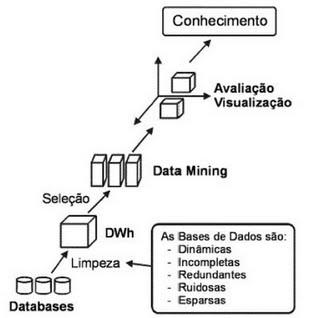
\includegraphics[scale=1.0]{exemplo_figura}
	
\end{figure}



	\chapter{Material e Métodos}
\section {Considerações Iniciais}
Essa é a área "Material e Métodos".

Nela, você deve discriminar o que foi adotado até o momento, ou prováveis métodos a serem usados para solucionar o problema. Indicar como e onde os dados serão obtidos


Abaixo, um exemplo de tabela, possivelmente útil nessa etapa do trabalho \ref{tb:tabela_dados}.

\begin{table}[htbp]
\caption{Exemplo de dados em tabelas}
\label{tb:tabela_dados}
\centering
\setlength{\tabcolsep}{5pt}
\begin{tabular}{cccccc}
\hline
Coluna 1  &Coluna 2  &Coluna 3 \\
L2Col1 &L2Col2 &L2Col3 \\
\hline
Dado1C1 &100 &200 \\
Dado2C1 &300 &400 \\
\hline
\textbf{Total} &\textbf{400} &\textbf{600} \\
\hline
\end{tabular}
\\
\text{\footnotesize Fonte: O autor}
\end{table}

\section{Exemplo de Código Fonte}
\subsection{ Teste de subseção}
Esse é um exemplo de código fonte ~\ref{code:exemplo_fonte}, que também pode ser útil nessa etapa do projeto de pesquisa.

%\lstset{frame=Trbl,numbers=left}
\begin{lstlisting}[caption={Exemplo de código fonte}, language=Python, label=code:exemplo_fonte]
	# Python program to check if the input number
	# is odd or even.
	# A number is even if division by 2 gives a
	# remainder of 0.
	# If the remainder is 1, it is an odd number.
	
	num = int(input("Enter a number: "))
	if (num % 2) == 0:
		print("{0} is Even".format(num))
	else:
		print("{0} is Odd".format(num))
\end{lstlisting}	


	\chapter{Conclusão}
%\setlength{\afterchapskip}{-\baselineskip}

\section {As transformações ocorridas na trajetória de pesquisa}
Reflexões em caso de alterações advindas da prática de pesquisa. Visão crítico-comparativa, Vantagens da soluções/métodos a serem adotadas, desvantagens e limitações


\section {Estágio atual da pesquisa}
Parte já desenvolvida da pesquisa. Indicação dos objetivos já atingidos e contribuições do trabalho
	\chapter{Cronograma}
Descrever em quadro dividido em meses, as atividades que necessitam ser executadas para a finalização do trabalho, indicando o período em que serão realizadas. 

No caso de coleta de dados em campo e/ou laboratório, indicar o período de coleta de dados.

Abaixo, um exemplo de cronograma \ref{fig:cronograma}.


\begin{figure}
	\caption{Exemplo de Cronograma - gantt}\label{fig:cronograma}
	\begin{gantt}{10}{12}
		\begin{ganttitle}
			\numtitle{1}{1}{12}{1}
		\end{ganttitle}
		\ganttbar{Revisão da literatura}{0}{2}
		\ganttbarcon{refinamento método}{2}{5}
		\ganttbarcon{}{8}{2}
		\ganttmilestone[color=cyan]{Milestone with color!}{4}
		\ganttbar{another task}{2}{2}
		\ganttbar[color=cyan]{another coloured task}{4}{4}
		\ganttbar{another task}{4}{2}
		\ganttcon{4}{5}{4}{7}
		\ganttmilestonecon{A connected Milestone}{7}
		\ganttbarcon{another consecutive task}{8}{2}
	\end{gantt}
	%\end{preview}
\end{figure}
	\chapter{Publicações resultantes do projeto}

Compreendendo o período desde a entrada no Programa até o presente
  
	
  
  
  
	\postextual
	%ljsenger - espaçamento entre o título e o primeiro parágrafo do texto
	\setlength\afterchapskip{18pt}
	%ljsenger - adeus a caixa alta
	\bibliographystyle{tcc-uepg}
	\bibliography{referenciasjabref}

% ----------------------------------------------------------
% Glossário
% ----------------------------------------------------------
%
% Consulte o manual da classe abntex2 para orientações sobre o glossário.
%
%\glossary

	% ----------------------------------------------------------
% Apêndices
% ----------------------------------------------------------

% ---
% Inicia os apêndices
% ---
\begin{apendicesenv}
	
	% Imprime uma página indicando o início dos apêndices
	%\partapendices
	
	\renewcommand{\thetable}{\Alph{chapter}\arabic{table}}
	\setcounter{table}{0}
	\clearpage
		\begingroup%
		\makeatletter%
		\let\clearpage\relax
		\vspace*{\fill}%
		\vspace*{\dimexpr-50\p@-\baselineskip}
		\chapter{EXEMPLO DE APENDICE}
		% inserir aqui o texto do apendice via \input{}
		\vspace*{\fill}%
		\endgroup 
	\clearpage

	% ----------------------------------------------------------
	
	Texto do apendice. Lembre-se: apendices são materiais elaborados pelo próprio autor.
	
	
\end{apendicesenv}
% ---
	
% ----------------------------------------------------------
% Anexos
% ----------------------------------------------------------

% ---
% Inicia os anexos
% ---
\begin{anexosenv}
	
	% Imprime uma página indicando o início dos anexos
	%\partanexos
	
	% ---
	\chapter{Exemplo de Anexo}
	% ---
	Texto do apendice. Lembre-se: anexos são materiais que não foram elaborados pelo próprio autor. 
  
  São exemplos de anexos os comprovantes das publicações informadas na seção 8 desse documento.
		
\end{anexosenv}



%---------------------------------------------------------------------
% INDICE REMISSIVO
%---------------------------------------------------------------------
\phantompart
\printindex
%---------------------------------------------------------------------

\end{document}	
